\documentclass[a4paper,man,natbib]{apa6}

\usepackage[spanish]{babel}
\usepackage[utf8]{inputenc}
\graphicspath{ {images/} }
\usepackage{apacite}
\usepackage{graphicx}
\usepackage{ragged2e}


\begin{document}
\begin{titlepage}
    \begin{center}
        \vspace*{1cm}
        
        \textbf{Diseño de una aplicación móvil para el diagnostico primario, prevención, seguimiento y  recomendaciones relacionadas al síndrome del túnel del carpo}
        
        \vspace{0.5cm}
        
        \vspace{1.5cm}
        
        \textbf{Felver Dueñas, Oscar Cadena, Santiago Ruiz}
        
        \vfill
        
       Anteproyecto para la especialización en\\
        Ingeniería de Software
        
        \vspace{0.8cm}
        
        
\includegraphics[width=0.6\textwidth]{image1.png}
        
        Especilización en Ingeniería de Software\\
        Universidad Distrital Francisco José de Caldas\\
        Bogotá \\
        17 de Abril de 2016
        
    \end{center}
\end{titlepage}
\tableofcontents

\clearpage
\section{INTRODUCCIÓN}
\justify
Las aplicaciones para la salud con los dispositivos móviles Apps, representan herramientas que pueden cambiar resultados y que ayudan en gran medida  a cubrir las exigencias del auto control en determinados tipos de patologías, el objetivo ultimo de estas aplicaciones no es sustituir al medico o profesional de la salud si no dar un apoyo en el registro y control sobre la enfermedad, que ayuda a tomar decisiones sobre como se está manejando el paciente en términos de hábitos de vida, tratamiento y diagnósticos.

El síndrome del túnel carpiano es una patología que afecto los nervios de la muñeca y que normalmente se origina de actividades repetitivas como usar herramientas o los periféricos del computador. La prolongación de dicho síndrome varia claramente de unos países a otros y de unas generaciones a otras, lo que sugiere que se trata de una dolencia cultural.

%\clearpage
\section {TÍTULO Y DEFINICIÓN DEL TEMA DE INVESTIGACIÓN}
\textbf{Diseño de una aplicación móvil para el diagnostico primario, prevención, seguimiento y  recomendaciones relacionadas al síndrome del túnel del carpo}

\section{ESTUDIO DEL PROBLEMA DE INVESTIGACIÓN}
\subsection{Planteamiento del problema}
El síndrome del túnel carpiano (STC) es una neuropatía periférica que ocurre cuando el nervio mediano se comprime dentro del túnel carpiano, a nivel de la muñeca. En relación a sus características epidemiológicas, el STC afecta aproximadamente $4\%$ de la población, con una incidencia anual entre 72 y 99 por cada 100000. \cite{s1} \cite{s4} Observando los factores de riesgo individuales para el STC, los resultados de casi todos los estudios de prevalencia sugieren que el STC es más frecuente en mujeres, con una incidencia anual de 1,5 por 1000 en comparación con 0,5 por 1.000 para los hombres. \cite{s5}  Las mujeres posmenopáusicas son comúnmente afectadas. \cite{s2}
El STC es causante de grandes costos para las empresas debido al pago de  incapacidades y pérdida de tiempo laboral por la recuperación de sus empleados. Algunos estudios han explorado los factores que están correlacionados con el retraso en el retorno al puesto de trabajo. Las características individuales, como la edad avanzada, el sexo femenino, la obesidad, trastornos musculoesqueléticos coexistente \cite{s6} y menor nivel de instrucción \cite{s7} han demostrado estar asociados de forma independiente con el retraso en el retorno al trabajo. Ahora, más allá del costo monetario, el paciente, puede llegar a perder su trabajo y muchas de sus capacidades motrices en su(s) mano(s) afectando de manera significativa su calidad de vida. Todo esto es causado por el poco cuidado que suelen tener las personas con su salud, aunado a que con la revolución tecnológica ahora muchos puestos de trabajo requieren de estar en una oficina en frente de un computador, entre otras labores, las cuales aumentan la presión en el nervio y los tendones medianos en el túnel carpiano propiciando el padecimiento del STC.
 Actualmente, Las aplicaciones móviles contribuyen en muchos aspectos a la vida de las personas, y aunque existen aplicaciones relacionadas con el síndrome del túnel carpiano, estas son en realidad incompletas y generalmente no superan una naturaleza informativa no validada científicamente. Adicionalmente, una buena parte de los diagnósticos de STC se deben al uso mismo de tecnologías, por lo cual una solución tecnológica, como lo es una aplicación móvil, implicaría para el usuario interactuar con una propuesta diferente de relación con estas herramientas,  que haga uso de sus facilidades y fortalezas de estas, sin desconocer su salud física.

\subsection{Formulación del Problema}

¿Cómo una aplicación móvil, puede ir mas haya de proveer simple información y convertirse en una herramienta que ayude a contrarrestar el síndrome del túnel Carpiano, incluyendo un diagnostico simple y ejercicios que permitan al usuario mejorar su calidad de vida y prevenir la posible aparición de la neuropatía periférica?

\subsection{Sistematización}
\begin{enumerate}
\item ¿Podemos sintetizar la información de importancia en una aplicación móvil de manera que el usuario entienda de manera sencilla pasos a seguir para sus ejercicios recomendados?
\item ¿Es posible que podamos medir la mejora en la calidad de vida de un paciente de STC gracias a la aplicación móvil?
\item ¿Qué ejercicios sencillos podemos utilizar que sean adaptables a ser mostrados por medio de una aplicación móvil y que sean realmente útiles tanto en la prevención como mejora del STC?
\item ¿Se puede en un medio sencillo y practico hacer un diagnóstico primario de STC por medio de una aplicación móvil?
\item ¿Podremos crear conciencia en las personas del STC?

\item ¿En el caso de Ingeniería de Software, se puede usar este primer desarrollo de modo que se puedan añadir extensiones de otras enfermedades?
\end{enumerate}

\section{OBJETIVOS DE LA INVESTIGACIÓN}
\subsection{Objetivo general}

\begin{itemize}
\item Diseñar un aplicativo basado en tecnologías móviles, encapsulando información medica confiable,que permita el diagnostico primario, seguimiento y recomendaciones relacionadas al síndrome del túnel del carpo.
\end{itemize}

\subsection{Objetivos específicos}
\begin{itemize}
\item  Consultar expertos con experiencia en el campo medico, que apoyen el proceso investigativo y generen feedbacks en el desarrollo del prototipo funcional. 
\item Recolectar informacion medica acertada , veridica y medible haciendo  uso de plataformas tecnológicas modernas. 
que permitan el agrupamiento de conceptos objetivos y la proyección de diagnósticos acertados.
\item  Realizar un prototipo de aplicación móvil usando las tecnologías e información disponibles. 
para mostrar un producto que sintetice todo el proceso investigativo.
\end{itemize}

\section{JUSTIFICACIÓN DE LA INVESTIGACIÓN}
\subsection{Justificación práctica}
Si bien el Síndrome del Túnel del Carpo es una enfermedad del sistema osteomuscular que resulta en el dolor y el deterioro funcional de las extremidades superiores, producto de compresión del nervio mediano de la muñeca \cite{v1}, diferentes aproximaciones investigativas y disciplinares han identificado que el impacto del desarrollo de esta enfermedad excede el malestar individual, ya que su gran nivel de ocurrencia llega a interferir en sistemas productivos de diferente índole y tiene un impacto en los requerimientos y servicios que las instituciones de salud ofrecen. De esta manera, en el comportamiento de la enfermedad  profesional en Colombia se ha documentado que los diagnósticos que afectan el sistema músculo esquelético corresponden al $65\%$, siendo el Síndrome del Túnel de Carpo la primera causa de morbilidad profesional \cite{v2}, ya que, como lo documenta Sura \cite{f2},  el síndrome del túnel carpiano es considerado la primera causa de incapacidad en Colombia con el $30\%$ de los casos.
Así mismo, el desarrollo de este Proyecto responde a la comprensión y demanda identificada por el Sistema Legislativo Colombiano de reconocer la preservación y conservación de la salud de los trabajadores como una actividad de interés social y sanitario (Ley 9 de 1979), \cite{v3}, entendiendo que tal interés requiere precisamente del aporte de disciplinas y saberes que complementen y apoyen a las ciencias de la salud desde metodologías, tecnologías e instrumentos innovadores que tengan un impacto en la cotidianidad de las personas. Identificando que el desarrollo de instrumentos relacionados con el Síndrome del Tunel del Carpo, tal como se consolida el diseño del aplicativo móvil presentado en este documento, tiene un impacto en sujetos particulares, pero también en las empresas en donde laboran y en los sistemas de salud a los cuales están inscritos,   es relevante retomar que el abordaje de esta enfermedad exige un acompañamiento en sus diferentes niveles de manifestación, configurándose medidas de prevención, diagnóstico temprano y tratamiento \cite{v3}. En ese sentido, los componentes y diseño planteado para el aplicativo móvil responden y dan cuenta a estas demandas, prevaleciendo claramente un interés por la prevención de la enfermedad, buscando tener un impacto en una población diversa que abarca a hombres y mujeres que desarrollan actividades que involucran el uso repetitivo de los músculos de la mano y la muñeca, aunque se reconoce que epideológicamente la enfermedad tiene una prevalencia en las mujeres (con una relación 7:1 frente a los hombres) y en personas que pertenecen al grupo etario entre los 40 y 60 años \cite{v1} Adicionalmente, la naturaleza práctica de la herramienta que propone este proyecto parte de emplear la tecnología móvil y su innegable accesibilidad para generar un producto asequible en el momento que las personas lo requieran desde el lugar en el que se encuentran. De esta manera, el resultado de este trabajo será un prototipo funcional de aplicación que permitirá llevar a cabo una mejora en la calidad de vida de las personas relacionadas con el Síndrome del Túnel Carpiano porque lo están padeciendo o porque existe la presencia de factores de riesgo asociados a la enfermedad. Se presentará la posibilidad de  generar un diagnostico primario que permitirá al usuario conocer su situación actual y, dependiendo de este diagnóstico, la sugerencia de la necesidad de asistencia a un profesional especializado,  o el acceso a consejos y ejercicios prácticos de prevención (en el caso de las personas que no presenten el síndrome). Habrá también un pequeño modulo informativo para conocer más sobre la enfermedad. Acorde al uso progresivo y mantenido en el tiempo, el aplicativo, cumpliendo con ciertos estándares de ingeniería, le brindará al usuario la posibilidad de registrar cambios en los síntomas de la enfermedad, comparando diagnósticos generados en diferentes espacios temporales. 

\section{HIPÓTESIS DE TRABAJO}
El uso de tecnologías móviles en el diagnóstico , pronóstico y control del síndrome del túnel carpiano pueden mejorar sustancialmente el estilo de vida de los pacientes asociados a la enfermedad facilitando tareas de monitorización y seguimiento e incluso modificando sus hábitos.

Los pacientes que padecen enfermedades relacionadas al túnel del carpo , pueden mejorar sustancialmente su estilo de vida empleando sistemas de software que constantemente evalúen variables relacionadas a sus hábitos y generen feedbacks  evidenciados en recomendaciones médicas que contribuyan al mejoramiento y/o tratamiento del síndrome.



\section{MARCO DE REFERENCIA}
\subsection{Marco teórico}
Este Proyecto, se basa en el principio básico de la ingeniería en el cual se pone el conocimiento al servicio de la humanidad \cite{f1} ya que buscamos por medio de una aplicación móvil, entregar conocimientos para prevenir la aparición del STC, lo cual derivará en un aumento en la calidad de vida de muchas personas propensas por distintas razones a esta enfermedad. Es importante aclarar que el desarrollo de la aplicación móvil será para dispositivos conocidos como smartphones y nos limitaremos a que sean compatibles con el sistema operativo Android. El STC puede llegar a presentarse por muchas razones,  entre ellas algunas de carácter genético, la obesidad o incluso el embarazo \cite{f2} , también, y aunque no ha sido asociada científicamente a alguna actividad como digitar en un teclado, escribir, cocinar, tocar algunos instrumentos musicales, entre otras \cite{f2}, este es el punto donde nos enfocaremos, ya que muchas personas llegan a sufrir dolencias en sus manos por no tener en cuenta factores como tomar pausas en su trabajo, o realizar calentamientos. Pretendemos entonces, enfocarnos en esta población, con una herramienta que va a permitirles un diagnóstico primario y ejercicios recomendados, para ayudar a conservar su salud y poder seguir con sus actividades, por ejemplo, el campo laboral se ve altamente afectado por el STC, este es un tema ya muy preocupante, ya que a principios del nuevo milenio, el $27\%$  de las enfermedades laborales reportadas eran por STC, en ese momento se el gobierno, liderado por el entonces Ministro de protección social Diego Palacio se vio obligado a lanzar una campaña para frenar esta estadística que al año costaba alrededor de  billones de pesos \cite{f3}, la cual no rindió frutos, ya que luego se amplió al $30\%$ \cite{f2}, mirando un poco más lejos de las estadísticas empresariales, de los costos que se presentan, también se debe tener en cuenta el factor humano, la pérdida de dinero jamas se podra comprar con la pérdida de calidad de vida de la persona afectada por STC, incluso con los tratamientos y cirugías, no es lo mismo, se pierde la capacidad de realizar muchas acciones cotidianas afectando de manera muy fuerte a la persona con el problema.
El avance tecnológico ha contribuido en muchos aspectos positivos  a la humanidad, en especial en la parte referente a la Informática, por ejemplo, un smartphone, es una importante herramienta la cual es de uso común durante el diario vivir, acompañándonos en todo momento, en Colombia ya existe una importante cantidad de personas que pertenecen a este grupo \cite{f4} y son también las asociadas con el STC, ya que este síndrome si bien no es nuevo, se a incrementado por el mismo avance tecnológico, por lo cual, queremos, haciendo uso de la tecnología, afrontar este tema, donde el smartphone será la herramienta que nos permita concientizar a las personas del STC, generar un diagnóstico primario y apoyarlos con una serie de ejercicios recomendados. Una encuesta reciente de la Sociedad Americana de Cirugía de la Mano comparó la práctica actual de sus miembros en relación al STC dónde noventa por ciento de los cirujanos utilizan pruebas de electrodiagnóstico ( EDT ) para confirmar STC antes de la operación. La descompresión del túnel carpiano se hacía típicamente a través de una incisión de mini- abierta ( $50\%$ ) bajo una anestesia local con sedación intravenosa ($43\%$). \cite{s3}
\subsection{Marco conceptual}
\begin{itemize}
\item Ingeniería de Sistemas.
La Ingeniería de Sistemas es la encargada de encontrar soluciones prácticas a la vida cotidiana a través de conocimientos matemáticos y ciencias de la ingeniería apoyados en la informática. \cite{f5}
\item Ingeniería de Software.
Ingeniería de software es el área de la ingeniería que ofrece métodos y técnicas para desarrollar y mantener software.
Esta ingeniería trata con áreas muy diversas de la informática y de las ciencias de la computación, tales como construcción de compiladores, sistemas operativos, o desarrollos Intranet/Internet, abordando todas las fases del ciclo de vida del desarrollo de cualquier tipo de sistemas de información y aplicables a infinidad de áreas: negocios, investigación científica, medicina, producción, logística, banca, control de tráfico, meteorología, derecho, Internet, Intranet, etc. \cite{f6}
\item Software.
Conjunto de programas, instrucciones y reglas informáticas para ejecutar ciertas tareas en un dispositivo con el hardware apropiado. \cite{f7}
\item Sindrome del Tunel Carpiano(STC).
El síndrome del túnel carpiano se produce cuando el nervio mediano, que va desde el antebrazo hacia la mano, se comprime o se aprieta en la muñeca. El nervio mediano controla las sensaciones del lado palmar del pulgar y los dedos (aunque no el meñique), al igual que impulsos a algunos músculos pequeños en la mano que permiten que se muevan los dedos y el pulgar. \cite{f8}.

\item Tunel Carpiano.
Un corredor rígido y estrecho de ligamento y huesos en la base de la mano, aloja al nervio mediano y los tendones. A veces, el engrosamiento de tendones irritados u otra inflamación estrecha el túnel y causa que se comprima el nervio mediano. El resultado puede ser dolor, debilidad, o entumecimiento en la mano y la muñeca \cite{f8}.

\item Nervio Mediano.
Nervio Sensitivo motor que inerva la mayor parte de la musculatura de anterior del antebrazo y región tenar, además suple la sensibilidad de la mano en su mitad radial, los tres primeros dedos y la cara radial del cuarto dedo. \cite{f9}

\item Síndrome.
Conjunto de signos y síntomas de causas diversas. \cite{f9}

Los síntomas del STC generalmente presentan una larga evolución, siendo los mas frecuentes: \cite{f9}
\begin{itemize}
\item Dolor en la cara palmar de la muñeca, que puede irradiarse a todo el territorio del nervio mediano.
\item Sensación de paso de corriente o quemadura en toda la mano.
\item Parestesias de las manos.\footnote{La parestesia es una condición donde una parte del cuerpo, generalmente un pie o una mano, comienza a sentir un hormigueo y se adormece}
\item Debilidad o adormecimiento de las manos.
\item Piel seca, edemas o cambios en la coloración de las manos.
\item Mejoría de los síntomas al cambiar la posición de la mano o sacudir la muñeca.
\item Disminución de la fuerza muscular e imposibilidad para manejar objetos pequeños y realizar actividades finas de la mano.
\item Cambios en la sensibilidad al tacto y/o temperatura.
\end{itemize}
\item Diagnóstico
Un examen físico de las manos, brazos, hombros y cuello puede ayudar a determinar si las quejas del individuo están relacionadas con las actividades diarias o con un trastorno subyacente. La muñeca se examina para detectar dolor, inflamación, calor y decoloración. Debe probarse la sensación de cada dedo, y los músculos en la base de la mano deben examinarse para evaluar la fuerza y los signos de atrofia. Los médicos pueden usar pruebas específicas para intentar producir los síntomas del síndrome del túnel carpiano. En la prueba de Túnel, el médico golpetea o presiona sobre el nervio mediano en la muñeca de la persona. La prueba es positiva cuando se produce hormigueo en los dedos o una sensación parecida a un shock. La prueba Phalen, o de flexión de la muñeca, implica hacer que la persona sostenga sus antebrazos verticales apuntando los dedos hacia abajo y presionando juntos los dorsos de las manos. La presencia del síndrome del túnel carpiano se sugiere si uno o más síntomas, como hormigueo o aumento del entumecimiento, se sienten en los dedos en 1 minuto. Los médicos también pueden pedirles a las personas que intenten hacer un movimiento que produzca los síntomas.A menudo es necesario confirmar el diagnóstico usando pruebas de electrodiagnóstico. \cite{f8}.

\item Tratamiento STC
Generalmente el tratamiento inicial implica descansar la mano y la muñeca afectadas durante al menos 2 semanas, evitando actividades que puedan empeorar los síntomas, e inmovilizando la muñeca con una tablilla para evitar mayor daño al girarla o doblarla. 
\item Tratamientos no quirúrgicos.
En circunstancias especiales, diversos medicamentos pueden aliviar el dolor y la inflamación asociados con el síndrome del túnel carpiano. Los medicamentos antiinflamatorios no esteroides, como la aspirina, el ibuprofeno, y otros analgésicos de venta libre, pueden aliviar los síntomas que han estado presentes por poco tiempo o que fueron causados por una actividad agotadora.
\item Ejercicio.
Los ejercicios de estiramiento y fortalecimiento pueden ser útiles en las personas cuyos síntomas han disminuido o terminado.
\item Terapias alternativas.
La acupuntura y la quiropráctica han beneficiado a algunas personas pero su eficacia sigue sin probarse. Una excepción es el yoga, que se ha demostrado que reduce el dolor y mejora la fuerza de agarre entre personas con el síndrome del túnel carpiano.

\item Cirugía.
La liberación del túnel carpiano es uno de los procedimientos quirúrgicos más comunes en los Estados Unidos. Generalmente, se recomienda la cirugía si los síntomas duran por 6 meses o si hay evidencia de daño muscular en casos graves del síndrome del túnel carpiano. La cirugía implica cortar la banda de tejido alrededor de la muñeca para reducir la presión sobre el nervio mediano.

\end{itemize}


\section{ESTADO DEL ARTE}
\subsection{Epidemiologia }
 
Actualmente los desordenes musculo esqueléticos representan una de las causas mas frecuentes de dolor crónico y ausencia de trabajo \cite{o1}, aproximadamente el 9,4 de las enfermedades musculo esqueléticas de la extremidades superiores están localizadas en el área de la muñeca y de las manos, de las cuales el síndrome del túnel de carpo representa el 1,5 \cite{o2}Colombia ligada al ambiente laboral, el síndrome del túnel carpiano es considerado la primera causa de incapacidad en Colombia (con el 30 de los casos)\cite{f2}. El STC (síndrome del túnel carpiano) es una costosa patología que afecta a jóvenes y adultos . La masificación de la tecnología a propiciado un crecimiento exponencial en el padecimiento de la enfermedad y los rangos de prevalencia pueden oscilar entre el 1 y el 5 de la población en general .Las oscilaciones pueden tener altos picos y subir incluso hasta un 14,5  en determinados grupos de trabajadores o personas que ejecutan actividades muy particulares asociadas a la manipulación repetitiva de elementos que requieren un uso prolongado de las extremidades superiores \cite{o1}.

En el 2010 la asociación colombiana para el estudio del dolor (ACED) presento los resultados del quinto estudio colombiano sobre el dolor, el cual tuvo énfasis en el dolor musculo esquelético y cuyo objetivo pretendía  la identificación de variables de percepción asociadas al dolor , las zonas del cuerpo de mayor afección y el efecto en las actividades de la vida diaria , social y laboral. La muestra para el estudio se conformo con 1.011 personas ,los resultamos identificaron que el 60 de la población investigada había padecido dolor musculo esquelético y que de acuerdo a la ocupación y esfuerzo realizado en su trabajo los más afectados eran los relacionados a trabajos de oficina con un 64 ,también se determino que los hábitos de vida son la causa más frecuente de las afecciones con un 91.6 de los casos .\cite{o5}

 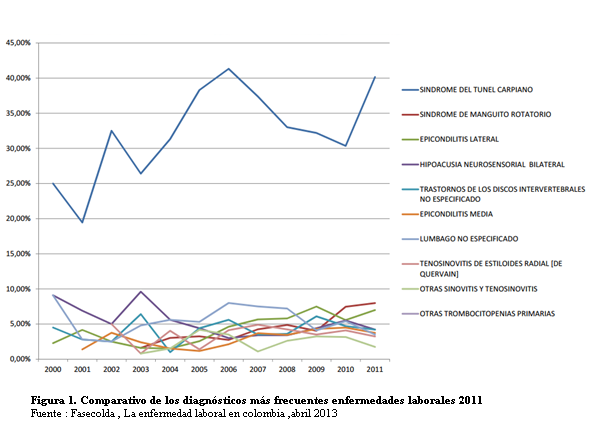
\includegraphics[width=0.99\textwidth]{grafica_1.png}
 
\subsection{Diagnostico Y Pronostico}

Los síntomas del STC son variables y van directamente relacionados a las severidad del estado compresivo y la presencia de  enfermedades coexistentes [6].Generalmente, produce dolor, hormigueo, sensación de quemadura, entumecimiento y alguna combinación de estos  síntomas en la región palmar del dedo pulgar, dedo índice, dedo medio y mitad radial del dedo anular \cite{o7}\cite{o8}\cite{o9}. Con la ayuda de un diagrama de la  muñeca un paciente puede localizar los síntomas , evidenciando una sensibilidad de 61 Y una especificidad de 71 para el diagnóstico \cite{o11}. Regularmente, los pacientes reportan que deben sacudir la mano afectada cuando los síntomas son severos. Muchos test de movimiento anatómicos pueden ayudar al diagnostico del síndrome. En el movimiento de Phalen, después de que el paciente flexione la muñeca por 60 segundos, el paciente refiere dolor o molestias en las áreas de  del nervio mediano\cite{o12}.Tiene una sensibilidad de 68 y una especificidad de 73 \cite{o13}. El signo de Tinel es más específico para el daño causado  por el STC en un nivel moderado a severo \cite{o14}\cite{o15}; es positivo, si al percutir suavemente sobre la cara volar de la muñeca se presenta  adormecimiento  hacia los dedos inervados por el nervio mediano. Éste tiene una sensibilidad de 50 y una especificidad de 77.En el examen de  provocación de presión, el pulgar del examinador es presionado sobre el túnel del carpo por 30 segundos \cite{o16}. En el del torniquete, se infla un  brazalete alrededor del brazo, por encima de la presión arterial , durante 60 segundos. Ambos exámenes se consideran positivos si desencadenan  molestias o adormecimiento en las áreas de inervación del nervio mediano.

\subsection{Tecnologías móviles en la salud}
La tecnología moderna ha revolucionado la forma en que la personas acceden a la información pasando de tener fuentes limitadas a tener una gran cantidad de fuentes de información con sólo un movimiento de dedo lo que subsecuentemente ha dado a los profesionales sanitarios la capacidad de combinar sus recursos de información y comunicación en un sólo instrumento portátil y a los pacientes la posibilidad de mejorar su estilo de vida mediante el control autónomo , diagnostico primario y educación preventiva de enfermedades\cite{o17} . Se estima que en Colombia hay aproximadamente 14.4 millones de usuarios de Smartphone \cite{o18} , y en este contexto un uso importante de dichos dispositivos es que pueden ser un elemento fundamental tanto para profesionales de la salud como para pacientes . un reciente articulo sobre el desarrollo y evaluación de aplicaciones móviles resalto lo grandes beneficios que puede acarrear el uso de dichas tecnologías tanto en profesionales de la salud como en pacientes, permitiendo tomar decisiones de manera mas rápida y con una menor tasa de error facilitando la gestión y la accesibilidad a los datos. Las "health apps" son destinadas al tratamiento y seguimiento de  dietas, balance energético, consejos, ejercicios, etc. Un estudio denominado  "patient apps for improving healthcare" \cite{o19}, publico los resultados de uno de los análisis más completos hasta la fecha enfocado a las aplicaciones móviles para el área de la salud. Este estudio analizó 43.689 apps y los resultados fueron que 20.007 (45,8) no estaban realmente relacionadas con la salud, eran más bien "trucos" sin unos beneficios reales; 7.407 (16,9) eran fiables, y estaban dirigidas a profesionales; 16.275 (37,3) eran fiables, y dirigidas a pacientes. pese a que aproximadamente el 50 de las aplicaciones se consideraban fiables, la mayoría de dichas aplicaciones eran simplemente  fuentes de información (no diferente a las encontradas en libros, revistas especializadas o internet).



\section{ASPECTOS METODOLÓGICOS}
A través de la identificación de los factores claves en la investigación, se estudiará de manera adecuada el tema de investigación para poder cumplir con los objetivos, vamos a definir  el tipo de investigación para el desarrollo del aplicativo móvil teniendo en cuenta entre otras cosas, técnicas de recolección de información y como se deberá tratar.

\subsection{Tipo de estudio descriptivo}
Debemos conocer las características del problema, con el fin de conocer su contexto para delimitarlo y plantear la solución,  Debemos conocer en forma detallada algunos de los aspectos del STC, por ejemplo, si queremos dar un diagnóstico primario, que tipo de test podemos aplicar al usuario que sea lo más parecido a   una consulta con un profesional, garantizando la veracidad de la información, y al mismo tiempo, identificando en qué momento, se debe aconsejar ir directamente con un especialista, en especial cuando sea necesario aplicar  pruebas de alta exactitud, como por ejemplo las pruebas de electrodiagnóstico \cite{f8}. Un factor importante, es comprender que las personas no suelen saber explicar bien lo que sienten en el caso de una enfermedad, las respuestas son ambiguas y si esto sucede con un profesional al frente de ellos, será también un aspecto a considerar para la aplicación móvil. 
Luego del Diagnóstico, es necesario realizar el análisis pertinente y ofrecer el mejor consejo posible, planteamos sobretodo dos escenarios posibles, en el que la persona se encuentra en un estado de STC realmente avanzado y es necesario acudir lo más pronto posible con un especialista, o bien, un panorama mejor, donde no se presentan o ninguno o muy pocos síntomas y se podrán recomendar ejercicios, que ayudaran en algunos casos a mejorar y sobretodo, prevenir que el síndrome aparezca.

\subsection{Método de Investigación}
Para conseguir los objetivos propuestos, debemos realizar una investigación adecuada, más aún en este caso, que se encuentra la salud y calidad de vida de una persona de por medio, primero, es necesario conocer al usuario final, quienes están propensos a padecer del síndrome así como tener contacto con la población que ya fue afectada y no tuvo otro remedio que someterse a la cirugía y su dolorosa recuperación, también,   hay que comprender  el tema que estamos tratando, investigar sobre el STC y tener una idea lo suficientemente clara como para demostrar un dominio del tema y poder de este modo, obtener una asesoría con un profesional con experiencia en el tema, que nos muestre un poco más cómo es que toda la teoría que ya debemos manejar se lleva a la práctica, allí encontraremos el escenario que nos va a permitir definir los requerimientos del software  y también la mayor veracidad posible de la información que este va a suministrar, siendo consientes en que casos y a que población podemos apoyar  y cuando hay que remitirse directo con un especialista.

entonces, tendremos que plasmar, tanto las inquietudes que tengamos por parte de los usuario, como los consejos por parte del profesional en el tema, con el fin de garantizar tanto que la aplicación será usada correctamente, como que está realmente prestará una ayuda.

\subsection{Fuentes y Técnicas para la recolección de la información}
Tenemos dos fuentes principales de información, primero, los posibles usuarios y segundo el especialista médico, entonces, al usuario final, con métodos de encuestas buscaremos conocer qué tan interesado está en usar la aplicación y cómo le gustaría que esta llegara a concientizar, no nos sirve de nada tener un excelente diagnóstico y recomendaciones si no logramos interés en la persona involucrada,   luego, según la información investigada y aclarada con el especialista, realizaremos un checklist de que se deberá incluir y luego presentaremos un feedback  mostrando los avances y que podemos mejorar, incluir o definitivamente descartar, de este modo contaremos con una herramienta atractiva y a la vez que cumple con su objetivo.

\subsection{Tratamiento de la Información}
Teniendo en cuenta, que la información que suministre la aplicación, no es solo su aspecto más importante, sino que al ser un tema sobre salud, es obligatorio saber que presentamos información verídica, en la que se pueda confiar, por lo tanto. abordando las dos fuentes de información tendríamos primero que todo, conocer con profundidad el tema para saber cómo presentarlo, además de contar  con una opinión experta, que garantice la mejor de las experiencias en el diagnóstico, así como  consejos que sean acertados, permitiendo una prevención del STC,   por otra parte, así como es importante la confiabilidad en la información, es importante saber presentarla, de manera amigable, para que el usuario le saque el mayor provecho, utilizando los mejores métodos en  el desarrollo de software, para tener una aplicación amigable y lista para que se puedan realizar posibles cambios.

\section{Cronograma de Trabajo}
\subsection{Diagrama de Gant}


\bibliography{mybib}
\bibliographystyle{plain}


\end{document}
